\documentclass[11pt]{article}

%%%%%% better tables
% install in R: reporttools and stargazer


\usepackage{longtable} % for tables

\usepackage{adjustbox} % for size



% TITLE , but needs to be 'made' (see below)

\title{My first replicable Paper}
\author{
        MyFirstName MyLastName\\
        Evans School of Public Policy and Governance\\
        University of Washington\\
        Seattle, WA 98115, \underline{United States}\\
        \texttt{greatguy@uw.edu}
}
\date{\today}


% notice \begin...\end
\usepackage{Sweave}
\begin{document}
\Sconcordance{concordance:PaperInR_6.tex:PaperInR_6.Rnw:%
1 26 1 1 0 31 1 1 6 1 1 1 7 8 1 1 8 29 0 1 2 13 1 2 2 14 1 1 8 14 0 1 2 %
5 1 2 2 18 1 2 2 16 1 2 2 11 1 1 2 4 0 1 2 2 1 1 2 4 0 1 2 1 1 1 2 23 0 %
1 2 1 1}


\maketitle % this will use the previous information. Do NOT MOVE.

% an abstract, notice \begin...\end

\begin{abstract}
This is an example on how to make a reproducible paper. We are using R from Rstudio, creating an RSweave document. This is a nice start to create a nice paper and get an A+. The next sections will show the steps taken.
\end{abstract}

% a section, notice it has a label for easy 'referencing'
\section{Introduction}\label{intro}  %if no numner were needed \section*

This is my intro to my great paper, I will explain the cool things I can do with my new `computational thinking' powers combined with some Latex. This is my intro to my great paper, I will explain the cool things I can do with my new `computational thinking' powers combined with some Latex. This is my intro to my great paper, I will explain the cool things I can do with my new `computational thinking' powers combined with some Latex. This is my intro to my great paper, I will explain the cool things I can do with my new `computational thinking' powers combined with some Latex.

% the newlines are not read:
This is my nice intro to my great paper, 
I will explain the cool things 
I can do with my new `computational thinking' 
powers
combined with some Latex.


\section{Exploring Data}\label{explo}

% footnotes, italic with \emph and referencing:
Sections may use a label\footnote{In fact, you can have a label wherever you think a future reference to that content might be needed.}. This label is needed for referencing. For example the next section has label \emph{datas}, so you can reference it by writing: As we see in section \ref{catexplo}.


%%%%%% code for loading here




\subsection{Exploring Categorical Data}\label{catexplo}

Here, I continue doing this nice work, I hope you like it and read it. It has been a very hard work.Here, I continue doing this nice work, I hope you like it and read it. It has been a very hard work.Here, I continue doing this nice work, I hope you like it and read it. It has been a very hard work.Here, I continue doing this nice work, I hope you like it and read it. It has been a very hard work.Here, I continue doing this nice work, I hope you like it and read it. It has been a very hard work.Here, I continue doing this nice work, I hope you like it and read it. It has been a very hard work.

You can see the statistics of categorical variables in Table \ref{catexplore_table}.

%%%%%% NEW VERSION

% latex table generated in R 3.5.2 by xtable 1.8-3 package
% Fri Feb 15 11:45:41 2019
\begingroup\normalsize
\begin{longtable}{llrrr}
\caption{Freq Table} \\ 
 \textbf{Variable} & \textbf{Levels} & $\mathbf{n}$ & $\mathbf{\%}$ & $\mathbf{\sum \%}$ \\ 
  \hline
Region & Africa & 11 & 14.5 & 14.5 \\ 
   & Asia & 35 & 46.0 & 60.5 \\ 
   & Eurasia & 6 & 7.9 & 68.4 \\ 
   & Europe & 15 & 19.7 & 88.1 \\ 
   & NAmerica & 5 & 6.6 & 94.7 \\ 
   & Oceania & 1 & 1.3 & 96.0 \\ 
   & SAmerica & 3 & 4.0 & 100.0 \\ 
   \hline
 & all & 76 & 100.0 &  \\ 
   \hline
\hline
ONI & nd & 2 & 2.6 & 2.6 \\ 
   & ne & 41 & 54.0 & 56.6 \\ 
   & per & 8 & 10.5 & 67.1 \\ 
   & sel & 21 & 27.6 & 94.7 \\ 
   & sub & 4 & 5.3 & 100.0 \\ 
   \hline
 & all & 76 & 100.0 &  \\ 
   \hline
\hline
\hline
\label{catexplore_table}
\end{longtable}
\endgroup




%%%%%%

You can see this variable plotted in Figure \ref{catexplore_plot}

\begin{figure}[h]
\centering
\begin{adjustbox}{width=7cm,height=5cm}
%\begin{adjustbox}{width=7cm,height=5cm,clip,trim=0cm 2cm 0cm 0cm} 
%trimmimg: left,bottom, right,top
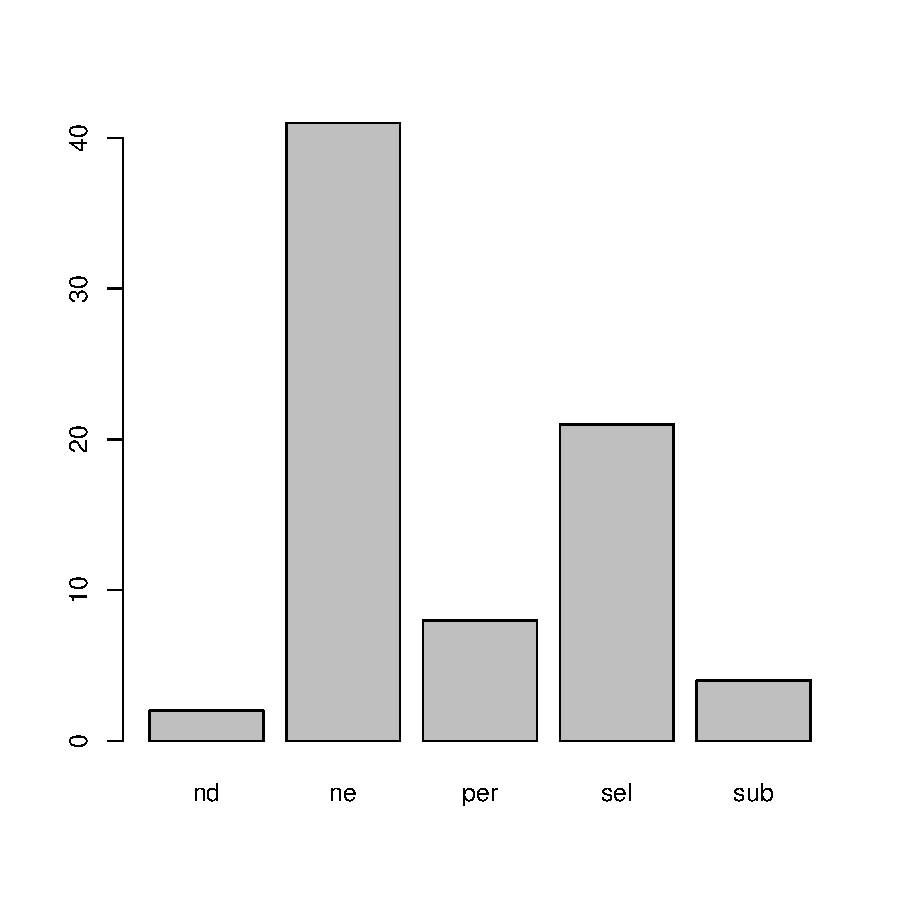
\includegraphics{PaperInR_6-catexplore_plot}
\end{adjustbox}
\caption{ONI barplot}  %title
\label{catexplore_plot} % for \ref{}
\end{figure}





\subsection{Exploring Numerical Data}\label{numexplo}

Here, I continue doing this nice work, I hope you like it and read it. It has been a very hard work.Here, I continue doing this nice work, I hope you like it and read it. It has been a very hard work.Here, I continue doing this nice work, I hope you like it and read it. It has been a very hard work.Here, I continue doing this nice work, I hope you like it and read it. It has been a very hard work.Here, I continue doing this nice work, I hope you like it and read it. It has been a very hard work.Here, I continue doing this nice work, I hope you like it and read it. It has been a very hard work.Here, I continue doing this nice work, I hope you like it and read it. It has been a very hard work.Here, I continue doing this nice work, I hope you like it and read it. It has been a very hard work.Here, I continue doing this nice work, I hope you like it and read it. It has been a very hard work.

%%%%%% code for exploring here

% Table created by stargazer v.5.2.2 by Marek Hlavac, Harvard University. E-mail: hlavac at fas.harvard.edu
% Date and time: Fri, Feb 15, 2019 - 11:45:41
\begin{table}[!htbp] \centering 
  \caption{Stat summary for nummeric vars} 
  \label{numexplore_table} 
\footnotesize 
\begin{tabular}{@{\extracolsep{5pt}}lccccccc} 
\\[-1.8ex]\hline 
\hline \\[-1.8ex] 
Statistic & \multicolumn{1}{c}{Median} & \multicolumn{1}{c}{Mean} & \multicolumn{1}{c}{Min} & \multicolumn{1}{c}{Max} & \multicolumn{1}{c}{Pctl(25)} & \multicolumn{1}{c}{Pctl(75)} & \multicolumn{1}{c}{St. Dev.} \\ 
\hline \\[-1.8ex] 
FH & 61 & 58.91 & 10 & 97 & 43.5 & 80 & 23.79 \\ 
RWB & 37.99 & 39.67 & 6.38 & 83.90 & 28.22 & 46.85 & 18.13 \\ 
\hline \\[-1.8ex] 
\end{tabular} 
\end{table} 
In the Table \ref{numexplore_table}, you realize that the mean of FH is {\bf58.9078947368421}.

\begin{figure}[h]
\centering
\begin{adjustbox}{width=7cm,height=5.5cm,clip,trim=0cm 1cm 0cm 0cm} 
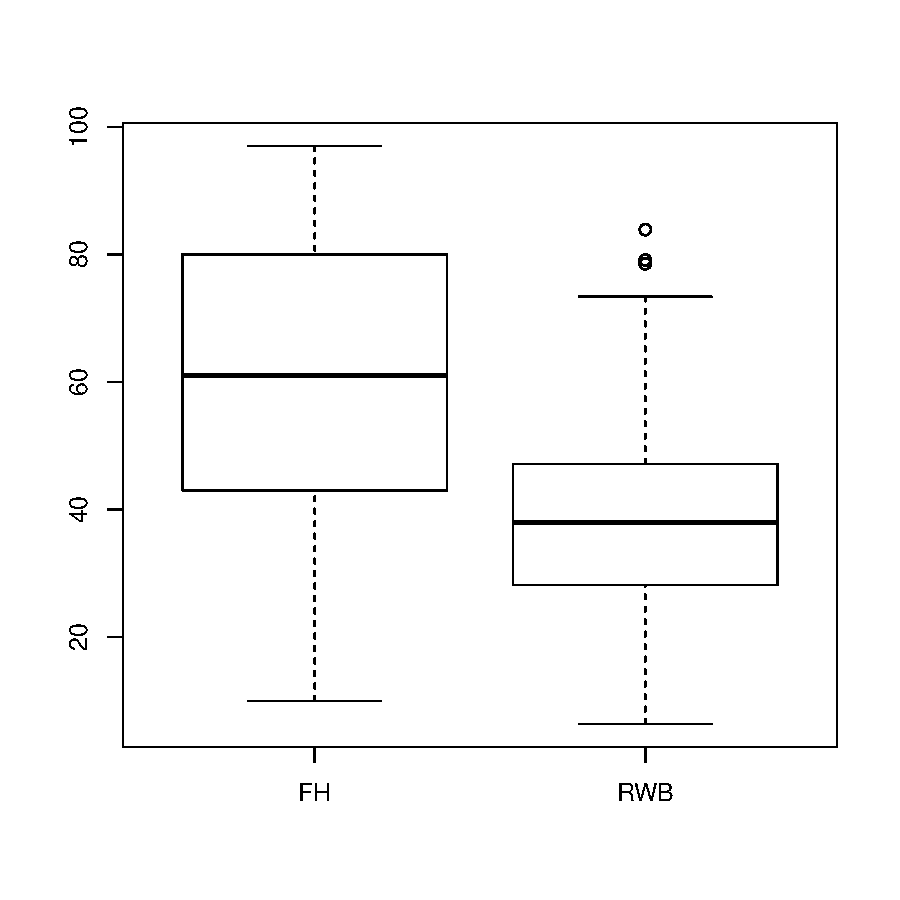
\includegraphics{PaperInR_6-numexplore_plot}
\end{adjustbox}
\caption{boxplots}  %title
\label{numexplore_plot} % for \ref{}
\end{figure}


Boxplots were introduced by Tuckey (Tukey, John W (1977). Exploratory Data Analysis. Addison-Wesley.)

\section{Looking for Relationships}\label{bivar}


Here, I continue doing this nice work, I hope you like it and read it. It has been a very hard work.Here, I continue doing this nice work, I hope you like it and read it. It has been a very hard work.Here, I continue doing this nice work, I hope you like it and read it. It has been a very hard work.Here, I continue doing this nice work, I hope you like it and read it. It has been a very hard work.Here, I continue doing this nice work, I hope you like it and read it. It has been a very hard work.Here, I continue doing this nice work, I hope you like it and read it. It has been a very hard work.Here, I continue doing this nice work, I hope you like it and read it. It has been a very hard work.Here, I continue doing this nice work, I hope you like it and read it. It has been a very hard work.Here, I continue doing this nice work, I hope you like it and read it. It has been a very hard work.

\subsection{Numerical and  Categorical}\label{binumcat}


\begin{figure}[h]
\centering                                  %trim=left,bottom,right,top
\begin{adjustbox}{width=7cm,height=7cm,clip,trim=0cm 0cm 0cm 0cm} 
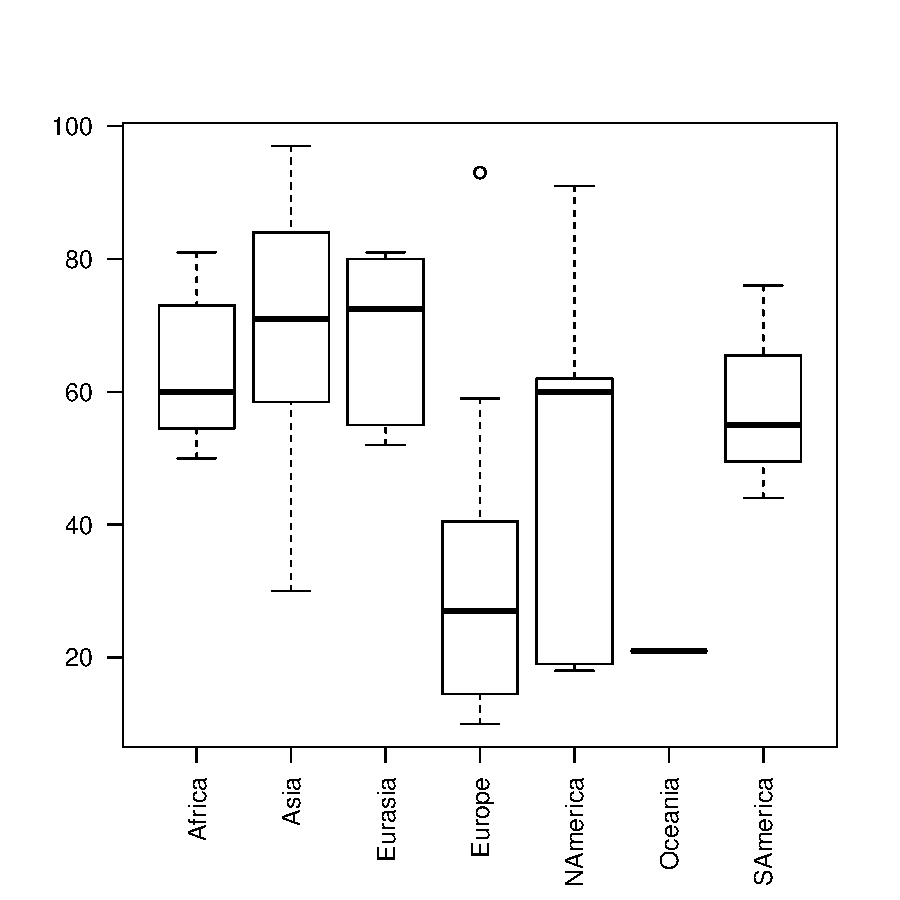
\includegraphics{PaperInR_6-numcat_plot}
\end{adjustbox}
\caption{boxplots}  %title
\label{numcat_plot} % for \ref{}
\end{figure}


Here, I continue doing this nice work, I hope you like it and read it. It has been a very hard work.Here, I continue doing this nice work, I hope you like it and read it. It has been a very hard work.Here, I continue doing this nice work, I hope you like it and read it. It has been a very hard work.Here, I continue doing this nice work, I hope you like it and read it. It has been a very hard work.Here, I continue doing this nice work, I hope you like it and read it. It has been a very hard work.Here, I continue doing this nice work, I hope you like it and read it. It has been a very hard work.Here, I continue doing this nice work, I hope you like it and read it. It has been a very hard work.Here, I continue doing this nice work, I hope you like it and read it. It has been a very hard work.Here, I continue doing this nice work, I hope you like it and read it. It has been a very hard work.

\subsection{Numerical and Numerical}\label{binumnum}

Here, I continue doing this nice work, I hope you like it and read it. It has been a very hard work.Here, I continue doing this nice work, I hope you like it and read it. It has been a very hard work.Here, I continue doing this nice work, I hope you like it and read it. It has been a very hard work.Here, I continue doing this nice work, I hope you like it and read it. It has been a very hard work.Here, I continue doing this nice work, I hope you like it and read it. It has been a very hard work.Here, I continue doing this nice work, I hope you like it and read it. It has been a very hard work.Here, I continue doing this nice work, I hope you like it and read it. It has been a very hard work.Here, I continue doing this nice work, I hope you like it and read it. It has been a very hard work.Here, I continue doing this nice work, I hope you like it and read it. It has been a very hard work.
%%%%%% code for exploring here


\begin{figure}[h]
\centering
\begin{adjustbox}{width=7cm,height=5.5cm,clip,trim=0cm 1cm 0cm 0cm} 
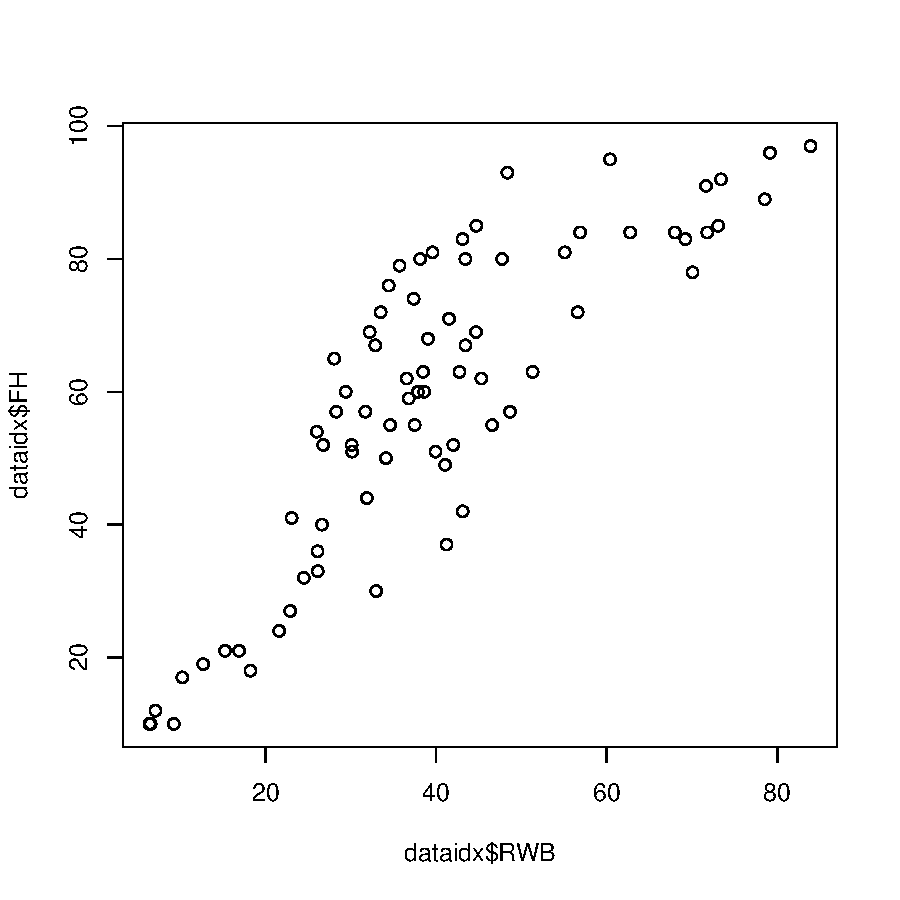
\includegraphics{PaperInR_6-numnum_plot}
\end{adjustbox}
\caption{boxplots}  %title
\label{numnum_plot} % for \ref{}
\end{figure}


The scatter plot is thought to be invented by  John Frederick W. Herschel according to this link: https://qz.com/1235712/the-origins-of-the-scatter-plot-data-visualizations-greatest-invention/

\section{My Regression}\label{regre}

This is a Regression in R:

\begin{Schunk}
\begin{Sinput}
> regre1=lm(FH~RWB,data=dataidx)
\end{Sinput}
\end{Schunk}

This is another:

\begin{Schunk}
\begin{Sinput}
> regre2=lm(FH~RWB+ONI,data=dataidx)
\end{Sinput}
\end{Schunk}

These is the traditional summary for one:
\begin{Schunk}
\begin{Sinput}
> summary(regre1)
\end{Sinput}
\begin{Soutput}
Call:
lm(formula = FH ~ RWB, data = dataidx)

Residuals:
    Min      1Q  Median      3Q     Max 
-23.631 -10.660  -2.094   9.858  24.501 

Coefficients:
            Estimate Std. Error t value Pr(>|t|)    
(Intercept) 14.75969    3.52175   4.191  7.6e-05 ***
RWB          1.11285    0.08084  13.767  < 2e-16 ***
---
Signif. codes:  0 ‘***’ 0.001 ‘**’ 0.01 ‘*’ 0.05 ‘.’ 0.1 ‘ ’ 1

Residual standard error: 12.69 on 74 degrees of freedom
Multiple R-squared:  0.7192,	Adjusted R-squared:  0.7154 
F-statistic: 189.5 on 1 and 74 DF,  p-value: < 2.2e-16
\end{Soutput}
\end{Schunk}

\end{document}
